\documentclass[10pt]{article}

\usepackage[margin=1in]{geometry}
\usepackage{amsmath,amssymb,booktabs,float,graphicx,microtype}
\usepackage[numbers,sort&compress]{natbib}
\usepackage[hidelinks]{hyperref}

\newcommand{\B}{\mathcal{B}}
\newcommand{\Oset}{\mathcal{O}}
\newcommand{\T}{\mathcal{T}}
\newcommand{\That}{\widehat{\mathcal{T}}}
\newcommand{\norm}[1]{\left\lVert #1 \right\rVert_{\infty}}

\title{Rate-Distortion Boundary Graphs for Auditable Semi-Markov Planning Compression}
\author{Anonymous authors}
\date{}

\begin{document}
\maketitle

\begin{abstract}
Planning in a finite Markov decision process repeatedly propagates reward
information through every primitive state, even when large regions have nearly
uniform control structure. We study whether such regions can instead be stored
as temporally extended edges between a small set of explicit states. We
introduce the RD Boundary Green Operator, a rate-distortion finite-difference
operator that scores which states must remain vertices using first-hit Green
kernels. For a fixed boundary, option family, and edge-weight model, the
operator is the exact finite difference of a local compression objective. A
one-shot implementation freezes the mandatory boundary and probe policies,
computes one truncated sparse Green response, thresholds a multichannel score,
and constructs the final graph kernels once; it performs no candidate
insertion or beam search. A group-constrained iterative fallback keeps
topological, value, and stochastic distortion budgets separate when the
one-shot graph fails an audit. Lean 4 proofs cover the frozen score identity, Green-kernel
legality and truncation bounds, graph-SMDP contraction, score certificates, and
an end-to-end decomposition from primitive optimal value to approximate graph
planning. On 12 classic map--slip cases, one-shot selection was a median
$40.1\times$ and $157\times$ faster than iterative surrogate and exact RD
search; after one final kernel build, the corresponding pipeline speedups were
$7.77\times$ and $22.9\times$. On 27 larger cases, it retained median
$192\times$ state compression with maximum normalized boundary-value gap
$0.00910$, but its total pipeline was only $0.00386\times$ as fast as matched
sparse value iteration because exact edge-kernel construction dominated. The
resulting claim is deliberately bounded: the method provides an auditable graph
abstraction for finite known-model SMDPs, not universal single-task acceleration
or a replacement for state abstraction and deep option learning.
\end{abstract}

\section{Introduction}
Dynamic programming over a finite Markov decision process (MDP) represents a
value at every primitive state and propagates task information through local
Bellman backups. This representation is appropriate when each state carries a
distinct control decision. It can be redundant in corridors, rooms, and other
regions where the important decision is which interface will be reached next.
In these settings, a compact planning model should retain the interface states
and represent the intervening region as a semi-Markov edge.

Options provide the standard formalism for temporally extended actions and
their induced semi-Markov decision processes (SMDPs)\citep{sutton1999options}.
Spectral option discovery uses graph geometry to propose useful directions or
subgoals\citep{machado2017laplacian}, while state abstraction and bisimulation
seek equivalence or controlled behavioral error\citep{li2006abstraction,ferns2011bisimulation}.
These approaches answer related but different questions. Option discovery asks
which extended actions to add; state aggregation asks which states may share an
abstract state. We ask which primitive states must remain explicit vertices so
that the rest of the MDP can be represented by first-boundary SMDP edges under
measurable rate and distortion constraints.

The central difficulty is not eliminating a fixed interior. A discounted Schur
complement gives an exact boundary model for each fixed option policy, analogous
to Kron reduction in graph and network models\citep{dorfler2013kron}. The hard
part is selecting the boundary without hiding task-relevant structure. A small
boundary may compress well but restrict control, bypass bottlenecks, or average
away a failure under one diagnostic lens.

We formulate boundary selection as a rate-distortion problem and derive the RD
Boundary Green Operator from first-hit kernels. The operator measures the local
decrease in hidden first-hit distortion caused by inserting a candidate state,
against the increase in graph description rate. Group constraints expose
topology, value-gradient, and transition-stochasticity failures separately. The
reference object is frozen: candidate universe, options, active edges, weights,
and rate costs are held fixed for one finite difference. The practical adaptive
solver may recompute these objects and is therefore not claimed to globally
optimize the frozen objective.

Our contributions are: (i) a Bellman-aware boundary-graph compression objective
based on exact first-hit option reductions; (ii) the frozen RD Boundary Green
Operator and a no-recompute, truncated sparse one-shot implementation; (iii) a
clear separation between that explicit operator, combinatorial reference
search, and a group-constrained adaptive fallback with an explicit
score-optimality boundary; (iv) an end-to-end value-gap decomposition that separates option restriction,
boundary restriction, kernel approximation, and planning residual; and (v) a
benchmark that compares option discovery, direct state abstraction, Schur/Kron
oracles, and strong full-state planners under matched constraints.

Figure~\ref{fig:pipeline} summarizes the claim boundary. The one-shot operator
replaces candidate search with one frozen message-passing transform, but the
returned graph is accepted only after explicit value and group audits. Failure
routes to adaptive group-constrained refinement rather than being hidden inside
the operator claim.

\begin{figure}[H]
\centering
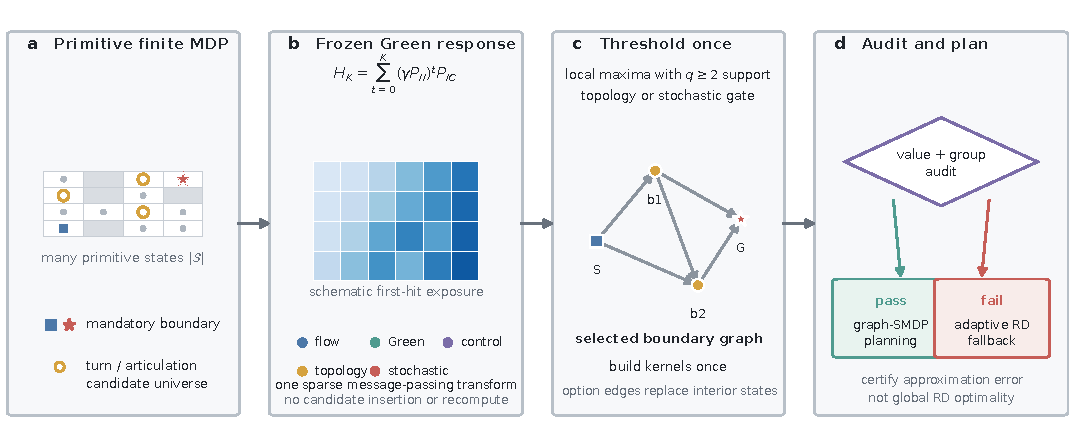
\includegraphics[width=\linewidth]{../experiments/output/operator_pipeline_figure/operator_pipeline.pdf}
\caption{The explicit no-recompute pipeline. A mandatory boundary and fixed
endpoint policies define one truncated first-hit Green response bank. Sparse
Laplacian, control, topology, stochastic, and exposure channels are normalized
and thresholded once to select additional vertices; no candidate is inserted
and rescored. Final first-boundary kernels are constructed once for the selected
graph. A passing graph is used for graph-SMDP planning, whereas a failed value or
group audit invokes adaptive group-constrained refinement. Green-tail and
selection-stability certificates bound approximation error; they do not make
the thresholded vertex set a global RD optimum.}
\label{fig:pipeline}
\end{figure}

\section{Related Work}
\paragraph{Temporal abstraction and option discovery.}
The options framework establishes that policies with initiation and termination
conditions induce SMDP models\citep{sutton1999options}; Option-Critic learns
option policies and terminations end to end\citep{bacon2017optioncritic}.
Laplacian option discovery instead derives task-independent eigenpurposes from
state-space geometry\citep{machado2017laplacian}. We use options as edge models,
but optimize which states remain graph vertices rather than treating option
discovery itself as the final objective.

\paragraph{Spectral graph operators.}
Localized spectral filters and graph convolutional networks turn Laplacian
polynomials or normalized adjacency operators into reusable message-passing
layers\citep{defferrard2016chebnet,kipf2017gcn}. This analogy motivates our
search-free implementation, but not its objective: a graph filter propagates an
observed signal, whereas the RD Boundary Green Operator scores whether an MDP
state must remain explicit using option-conditioned first-hit exposure, control
curvature, and rate cost. The random-walk Laplacian channels in the one-shot
transform are therefore computational components, not a claim that an ordinary
spectral cut preserves Bellman behavior.

\paragraph{State abstraction and model reduction.}
MDP homomorphisms, SMDP homomorphisms, and approximate abstractions formalize
when state distinctions can be removed\citep{ravindran2003smdp,li2006abstraction}.
Bisimulation metrics quantify behavioral similarity and connect model error to
value error\citep{ferns2011bisimulation}. Our experiments include homogeneous
partition refinement and reward-aware oracle aggregation as direct baselines.
State--option abstractions can also preserve near-optimal behavior under explicit
compatibility conditions\citep{abel2020valuepreserving}.
The proposed representation differs structurally: interior states are not
merged into one Markov state, but eliminated into option-labeled first-boundary
edges while a sparse interface remains explicit.

\paragraph{Schur reduction and information-theoretic compression.}
Kron reduction preserves boundary behavior of a graph Laplacian through a Schur
complement\citep{dorfler2013kron}. Our exact edge model is a discounted,
reward-bearing option analogue. Rate-distortion approaches motivate trading
model complexity against task loss\citep{arumugam2021rate,abel2019compression}.
We combine these views by using first-hit Green kernels to define where an
SMDP region should be split.

\paragraph{Learned planning graphs.}
Replay-buffer search, goal-conditioned planning, and latent-landmark world
models construct sparse graphs for long-horizon control
\citep{eysenbach2019sorb,nasiriany2019goalconditioned,zhang2021worldgraph}.
Their nodes and edges are generally learned from observations, reachability, or
goal-conditioned values. We instead begin with a finite transition model and
ask which interface states can be eliminated while retaining an auditable
first-boundary SMDP. The external-environment experiments test interface
portability, not parity with these deep representation-learning systems.

\paragraph{Successor representations and diagnostic residuals.}
Successor representations and successor features separate predictive dynamics
from reward weights, enabling transfer across reward functions under fixed
dynamics\citep{dayan1993successor,barreto2017successor}. Our fixed-boundary edge
occupancy kernel uses the same linear reward-relabeling principle, but is option
conditioned and stops at the next boundary. Conversely, a small Bellman error
need not imply a small value error\citep{fujimoto2022bellman}. This is why we
report normalized value gaps and a contraction-based residual-to-value bound
instead of treating a scalar residual as sufficient preservation evidence.

\section{Problem Formulation}
Let $M=(\mathcal{S},\mathcal{A},P,r,\gamma)$ be a finite discounted MDP with
$0\leq\gamma<1$. A boundary set $\B\subseteq\mathcal{S}$ contains task
terminals and the states retained as graph vertices. For each option
$o\in\Oset(b)$, let $\tau_\B$ denote the first positive hitting time of the
next boundary state. The exact boundary reward and continuation kernel are
\begin{align}
R^o_\B(b) &= \mathbb{E}_b^o\left[\sum_{t=0}^{\tau_\B-1}\gamma^t
r(S_t,A_t)\right],\\
\Gamma^o_\B(b,b') &= \mathbb{E}_b^o\left[\gamma^{\tau_\B}
\mathbf{1}\{S_{\tau_\B}=b'\}\right].
\end{align}
The graph-SMDP Bellman operator is
\begin{equation}
(\T_\B V)(b)=\max_{o\in\Oset(b)}\left[R^o_\B(b)+
\sum_{b'\in\B}\Gamma^o_\B(b,b')V(b')\right].
\end{equation}
For fixed $\B$ and $\Oset$, these kernels define the option-restricted SMDP
exactly. This statement does not imply equality to the primitive optimal MDP;
the option family may be insufficient.

We seek a small boundary that satisfies value and audit constraints. Writing
$\mathrm{Rate}(\B)$ for graph description cost and $D_g(\B)$ for the
distortion under diagnostic group $g$, the robust objective is
\begin{equation}
\min_{\B}\ \mathrm{Rate}(\B)\quad
\text{subject to}\quad D_g(\B)\leq\epsilon_g\ \ \forall g,
\quad \Delta_V(\B)\leq\epsilon_V.
\end{equation}

\section{The RD Boundary Green Operator}
\subsection{Exact first-hit reduction}
For one fixed option policy, partition its transition matrix into boundary and
interior blocks. The discounted continuation kernel is
\begin{equation}
\Gamma_\B=\gamma P_{BB}+\gamma^2P_{BI}
(I-\gamma P_{II})^{-1}P_{IB},
\end{equation}
and the reduced reward is
\begin{equation}
R_\B=r_B+\gamma P_{BI}(I-\gamma P_{II})^{-1}r_I.
\end{equation}
The undiscounted first-hit Green term
$P_{BI}(I-P_{II})^{-1}$ records interior visitation before the next boundary
hit. Its candidate columns determine how much active edge mass would be exposed
by inserting a new vertex.

\subsection{Frozen rate-distortion finite difference}
Let $L_\theta(\B)$ be a local objective whose parameters $\theta$ fix the
candidate universe, option library, active edges, edge weights, rate costs, and
diagnostic probes. The score of candidate $x$ is
\begin{equation}
S_{\mathrm{FD}}(x\mid\B)=L_\theta(\B)-L_\theta(\B\cup\{x\}).
\end{equation}
This is the RD Boundary Green Operator. Its distortion change is computed from
first-hit mass on edges affected by $x$; its rate term charges the inserted
vertex and edge interface. The frozen qualification is essential. Once an
outer solver rebuilds options, occupancies, or weights, it is optimizing a
sequence of related local objectives rather than one fixed set function.

\subsection{No-recompute one-shot implementation}
The finite-difference score above is a reference objective, but evaluating it
after every possible insertion is itself a combinatorial search. Our fast path
instead applies a fixed Green-derived transform once. Starting from mandatory
boundary $\B_0$ and a fixed anchor set $C$ (the task endpoints by default), let
$P^{(c)}$ be the sparse transition matrix of the fixed policy targeting anchor
$c$. The truncated response bank is
\begin{equation}
H_K(:,c)=\sum_{t=0}^{K}(\gamma P^{(c)}_{II})^tP^{(c)}_{Ic},
\end{equation}
and a discounted forward pass from each active source gives an exposure field
$u_K$. Both are sparse message-passing computations; they are not recomputed
for candidate insertions.

For every candidate state, one random-walk Laplacian application forms Green,
control-policy, and transition-entropy curvature channels. These are combined
with exposure and a fixed topology channel. After robust per-channel
normalization, the operator keeps eligible local maxima supported by at least
$q$ channels above threshold $\tau$, requires a topology or stochastic gate,
and retains at most $m$ states in a deterministic exposure-first order:
\begin{equation}
\B_{\mathrm{1shot}}=\B_0\cup
\operatorname{Top}_m\!\left(\operatorname{LocalMax}_{\tau,q}
(u_K,\mathcal L_{rw}H_K,\mathcal L_{rw}\pi,
\phi_{topo},\mathcal L_{rw}\mathsf H(P))\right).
\end{equation}
Only after this single selection is the exact or certified approximate graph
kernel built for the final $\B_{\mathrm{1shot}}$. Its discovery complexity is
$O(|C|K\,\mathrm{nnz}(P))$ plus sparse channel application, rather than one or
more Green solves per candidate and search step.

This transform is deliberately analogous to a fixed convolutional or graph
filter: it is motivated and calibrated by the exact RD finite difference, but
we do not claim that thresholding it globally minimizes the RD set objective.
Instead, Green-tail intervals certify channel error, score margins certify
threshold and local-maximum stability, and the returned graph is checked by
the same value and audit metrics as every other selector. Failed group audits
invoke the iterative fallback rather than being silently declared preserved.

\subsection{Group constraints and adaptive discovery}
A scalar risk can compensate a topology failure with a low value-gradient risk,
or vice versa. We therefore preserve separate topology, value, and stochastic
groups. The adaptive solver accepts a boundary only when every specified group
is feasible. Candidate scores are proposed in a frozen or surrogate order and
then refined exactly or with certified intervals.

Adaptive feasible top-$k$ scans this shared order and stops at the first
certified feasible candidate, up to cap $k$. Under a shared ordering and
feasibility oracle, it discovers a feasible candidate if and only if fixed
top-$k$ contains one, and it evaluates no more than $k$ candidates. This is a
feasible-envelope guarantee. Score-optimality additionally requires interval
dominance: the selected lower score bound must exceed every competing upper
bound.

\subsection{Certified Green approximation}
The inverse in the Green kernel can be replaced by a Neumann prefix,
\begin{equation}
(I-P_{II})^{-1}\approx\sum_{t=0}^{K}P_{II}^t.
\end{equation}
Adaptive truncation increases $K$ until a frontier-tail score interval is below
a requested tolerance. If intervals do not separate the leading candidate, a
top-set exact fallback is reported explicitly. Weighted Collatz certificates
provide a stronger sufficient convergence test when a raw row-sum condition is
too conservative; they are appendix certificates rather than the main runtime
decision rule.

We also test whether a graph-conditioned model can predict $K$ before message
passing. This prediction is only a scheduling proposal: the same frontier
certificate remains authoritative, and a failed proposal continues or falls
back. Consequently, learning changes runtime but not the certified acceptance
condition.

\section{Value Preservation Accounting}
Let $V^*$ be the primitive optimal value, $V^{\Oset}$ the value after restricting
the option/action family, $V^{\B,\Oset}$ the exact boundary-option value,
$\widehat V^{\B,\Oset}$ the approximate-kernel fixed point, and
$\widetilde V^{\B,\Oset}$ the computed value. If the exact and approximate
graph operators have contraction modulus at most $\beta<1$, then our Lean
certificate instantiates
\begin{align}
\norm{V^*-\widetilde V^{\B,\Oset}}
\leq{}& \epsilon_{\mathrm{option}}+\epsilon_{\mathrm{boundary}}\\
&+\frac{\epsilon_R+V_{\max}\epsilon_\Gamma}{1-\beta}
+\frac{\epsilon_{\mathrm{plan}}}{1-\beta}.
\end{align}
The four terms respectively measure option-family restriction, commitment to
the retained interface, reward/continuation-kernel approximation, and the final
planning residual. The theorem certifies the returned graph; it does not assume
that boundary discovery is globally optimal.

\section{Fixed-Boundary Multi-Task Rewards}
Promoting every possible reward or goal state into $\B$ destroys compression by
construction. For additive rewards, we instead store the discounted edge
occupancy kernel
\begin{equation}
M^o_\B(b,s)=\mathbb{E}_b^o\left[\sum_{t=0}^{\tau_\B-1}
\gamma^t\mathbf{1}\{S_t=s\}\right],
\end{equation}
so a new reward $r$ relabels the edge by
$R_r^o(b)=\langle M^o_\B(b,\cdot),r\rangle$ without changing $\B$.
Interior terminal goals require a separate first-hit event kernel. Their
remaining error is reported as option/boundary restriction bias; a
goal-conditioned local option family is an explicit, costed extension rather
than a hidden assumption.

\section{Experimental Protocol}
We evaluate corridors, open rooms, four-room maps, hand-designed mazes, and
random depth-first-search mazes under slip probabilities $0$, $0.05$, and
$0.1$. External finite-MDP tests include Gymnasium ToyText, symbolic MiniGrid,
and a discretized PointMaze. Taxi is retained as a structured negative case
because passenger and destination variables violate a purely spatial boundary
assumption.

Baselines include full synchronous and sparse-vectorized value iteration,
Gauss-Seidel value iteration, prioritized sweeping\citep{moore1993prioritized},
eigenoptions, betweenness bottlenecks, random and coverage landmarks,
homogeneous state aggregation, reward-aware $Q^*$ oracle aggregation, and a
policy-specific Schur oracle. Oracle baselines are labeled because they consume
the full optimal value or policy.

The primary comparison is an epsilon-constrained frontier. A row is eligible
only when normalized value gap, normalized audit distortion, success, and group
feasibility satisfy a common protocol. We then compare boundary rate,
compression, planning cost, and amortized cost. Full-state planners use five
matched repeats with medians, interquartile ranges, and per-case bootstrap
intervals. The legacy XL graph rows contain one construction measurement per
case; selector-level intervals therefore resample cases rather than repeated
graph construction. This is sufficient to establish the large negative
single-task result, but not a claim of systems-level runtime superiority.
Legacy Python VI timing is retained only for historical reproduction; claims
use the fastest numerically valid matched full-state planner.

Unless a sensitivity row states otherwise, the one-shot operator uses
$\gamma=0.97$, the mandatory task endpoints as two probe anchors, the union of
turn and articulation candidates, a one-hop exclusion around mandatory states,
a 256-step Green prefix with frontier tolerance $10^{-6}$, and per-graph
95th-percentile channel normalization. A candidate must be a local maximum in
at least two channels and must include topology or stochastic support. We retain
at most 18 candidates. The central threshold $\tau=0.15$ is the middle operating
point of the classic $\{0.10,0.15,0.20\}$ sensitivity sweep and is reused
unchanged on held-out random mazes and the XL suite. The production final-edge
builder uses certified adaptive first-hit truncation; the fixed 256-step prefix
is the frozen one-shot scoring transform.

\section{Results}
\subsection{Does the explicit one-shot operator replace search?}
The earlier RD Green surrogate row used iterative candidate insertion and
recomputed the boundary context after each split. Its single-task total-time
number therefore measured a search algorithm, not the fixed operator proposed
in the introduction. We implemented the no-recompute path separately and
instrumented it to report zero candidate-insertion evaluations, zero beam
expansions, one Green response per fixed anchor, and exactly one final graph
kernel build.

On 12 classic map--slip cases, the fixed threshold $\tau=0.15$ selected a
boundary in a median 0.01095 seconds. This was $40.1\times$ faster than the
iterative surrogate selector and $157\times$ faster than exact RD search on
the same cases. After charging one final graph-kernel build, paired median
speedups remained $7.77\times$ and $22.9\times$, respectively. The one-shot
boundary was modestly denser (median boundary-size ratio 1.25 relative to the
iterative selector). Its global maximum normalized value gap was unchanged at
0.00963, while median occupancy-weighted hidden distortion decreased from
0.380 to numerical zero. Boundary Jaccard agreement was 1 on corridor and most
maze cases, but only 0.5--0.667 on four-room and open-room cases; similar value
does not imply identical abstraction.

The held-out DFS-maze suite contains 108 size--seed--slip contexts for each of
two fixed thresholds. At $\tau=0.15$, median state compression was $6.30\times$,
maximum normalized value gap was $1.46\times10^{-7}$, and median occupancy
distortion was below $10^{-6}$. Raising the fixed threshold to 0.75 increased
compression to $9.70\times$ and left task value accurate, but raised median
occupancy distortion to 7.0. This is the intended rate--distortion behavior and
also shows why task value alone is an insufficient selection criterion.
On a paired 20-context subset (sizes 11 and 15, five seeds, and two slip
levels), one-shot and iterative-surrogate boundaries had median Jaccard 0.920.
One-shot extraction was $369.5\times$ faster and the complete graph pipeline
was $12.94\times$ faster, while maximum normalized value gaps were
$1.20\times10^{-7}$ and $1.08\times10^{-7}$, respectively.

On the 27-case XL map--slip suite, one-shot extraction took a median 0.0797
seconds and produced median $192\times$ state compression; maximum normalized
start and boundary-value gaps were 0.00784 and 0.00910. Relative to the legacy
iterative RD rows paired by map and slip, extraction was $947\times$ faster and
the full one-shot graph pipeline was $15.1\times$ faster. These cross-run ratios
diagnose algorithmic cost rather than constitute a repeated systems benchmark.
Against the matched sparse full-state planner, single-task total speedup was
still only $0.00386\times$: the median final-kernel build was 2.05 seconds,
whereas the explicit operator itself took 0.0797 seconds. Thus the original
operator idea works as a replacement for combinatorial boundary search, but it
does not by itself remove exact edge-kernel construction cost.

\begin{table}[H]
\centering
\caption{One-shot operator evidence at the fixed $\tau=0.15$ operating point.
``Extract/iter.'' compares boundary selection with paired iterative surrogate
search; ``graph/iter.'' also charges one final kernel build and graph solve.
``total/sparse'' compares that complete graph pipeline with sparse full-state
VI, so values below one expose the remaining single-task cost. The XL iterative
ratios pair separately generated rows by map and slip and are algorithmic-cost
diagnostics rather than repeated systems measurements.}
\label{tab:one-shot}
\footnotesize
\begin{tabular}{lrrrrrr}
\toprule
Suite & Cases & State comp. & Max norm. gap & Extract/iter. & Graph/iter. & Total/sparse\\
\midrule
Classic maps & 12 & 21.0 & 0.00963 & 40.1 & 7.77 & 0.0171\\
Held-out random & 20 & 4.85 & $1.20\!\times\!10^{-7}$ & 369.5 & 12.94 & 0.00573\\
XL maps & 27 & 192.0 & 0.00910 & 947.1 & 15.13 & 0.00386\\
\bottomrule
\end{tabular}
\end{table}

A trainable-horizon pilot used 105 training, 15 calibration, and 60 larger or
held-out graph--slip contexts. A ridge proposal with split-conformal upper
correction passed the certificate on its first attempt in 56/60 cases and after
fallback in 60/60; the minimum boundary Jaccard against adaptive truncation was
one. However, after charging graph-feature extraction and retries, its median
speedup was only $0.906\times$ relative to a fixed 256-step prefix and
$0.747\times$ relative to the existing adaptive frontier stop. Thus $K$ is
predictable, but learning a scalar horizon is not the useful single-graph
acceleration: the production implementation retains certified adaptive
truncation, while learned horizons are at most a batching/scheduling ablation.

\paragraph{Learned proposal ablations.}
We also tested whether graph-conditioned learning could replace the explicit
operator and its audit (Appendix~\ref{app:learned}). A boundary-only GCN passed
the strict held-out joint constraint in 68/90 contexts, compared with 62/90 for
nearest-start and 71/90 for the adaptive RD reference proposal. One predefined
constraint-aware follow-up reranked a frozen five-proposal family and increased
raw passes to 81/90, near the family oracle of 85/90, at $656\times$ selection
speed. This is metric-specific post-selection rather than operator dominance:
the reranker uses downstream risk labels and optimizes a different objective.

The safety gate rejected the learned path. Validation-calibrated routing found
only 3 of 9 scale-holdout failures, leaving six unaudited; full audit removed
those misses but reduced median pipeline speed to $0.428\times$ the adaptive RD
reference. The paired outcomes were 64 both-pass, 17 reranker-only, 7
reference-only, and 2 both-fail (exact McNemar $p=0.0639$). We report this
comparison descriptively, stopped the constraint-aware topology extension under
the predefined go/no-go protocol, and retain learning only as an uncertified
ablation.

The hard group audit is the main negative result. A frozen one-shot score did
not satisfy all topology/value/stochastic groups on the three-map diagnostic,
and adding more fixed local maxima did not monotonically repair feasibility
because the option library changes with the boundary. The stricter frozen
group finite-difference prefix confirms the mechanism:
open-room was feasible only at tested prefix $k=2$ and infeasible again at
$k=3$; four-rooms was feasible at tested prefixes $k=3,4,5,6,8,10$ but not
$k=12$; and maze had no feasible prefix through $k=24$. Thus even an exact
frozen candidate order neither guarantees feasibility nor induces a monotone
feasibility path under an adaptive option library.
We therefore use
one-shot as the primary proposal and task-value path, then expose audit failure
and invoke group-constrained refinement when required. We do not fold fallback
time into the one-shot operator measurement or claim universal MDP equivalence.

\subsection{Compression and constrained planning}
The XL suite contains 135 large-scale compression rows, 360 random-maze rows,
and 648 option-frontier rows. In five paired repetitions of each of 27
map--slip cases, sparse-vectorized VI was the fastest valid full-state planner;
its per-case medians and bootstrap intervals are therefore the runtime
denominator. Table~\ref{tab:strong-runtime} separates graph planning from
construction. The RD selector compressed the state representation by a median
$256\times$ and made graph planning $29.6\times$ faster, while its worst
normalized start gap was $0.00589$. Across cases, the bootstrap 95\% interval
was $[21.1,71.4]\times$ for graph planning. Nevertheless, its median
single-task total speedup was only $0.00116\times$ (95\% interval
$[0.000591,0.00159]\times$): discovery and kernel construction cost much more
than one sparse full-state solve. This row is the iterative surrogate-search
pipeline, not the one-shot operator above. It remains as the constrained
reference/fallback result and is not used to characterize one-shot extraction
cost. This is a planning-compression result, not a single-task wall-time win.

\begin{table}[H]
\centering
\caption{Large-scale medians against matched sparse-vectorized VI. Total time
includes discovery, kernel construction, graph planning, and tie-aware
fallback. Gap is normalized by the conservative discounted unit-reward bound
$1/(1-\gamma)$.}
\label{tab:strong-runtime}
\footnotesize
\begin{tabular}{lrrrr}
\toprule
Selector & State comp. & Max norm. gap & Plan speedup & Total speedup\\
\midrule
Endpoints & 256.0 & 0.00589 & 43.45 & 0.0121\\
Turn articulation & 128.0 & 0.00589 & 6.02 & 0.00332\\
Betweenness & 22.3 & 0.00589 & 0.0173 & 0.000473\\
Coverage & 22.3 & 0.00589 & 0.138 & 0.000435\\
RD Green surrogate & 256.0 & 0.00589 & 29.58 & 0.00116\\
\bottomrule
\end{tabular}
\end{table}

Under the canonical constraints $\epsilon_V=0.01$ and
$\epsilon_{audit}=0.001$, the large-scale RD graph was feasible in 13/27 cases
with median $288\times$ compression. Coverage landmarks were feasible in 21/27
but compressed only $24\times$; the dense turn graph covered 27/27 at
$128\times$. Thus no selector dominates: the useful result is the explicit
coverage--rate frontier. The artifact first reports constraint coverage, then
computes compression and bootstrap intervals on paired eligible cases. Legacy
dense-VI timings remain in the reproduction tables but are not used for the
strong-runtime claim.

\subsection{Direct abstraction and end-to-end error}
Exact homogeneous model minimization retained every state in the direct
baseline suite. Epsilon-homogeneous aggregation compressed by a median
$33\times$, but its median normalized start gap was $0.544$ and its maximum was
$0.846$. The policy-Kron oracle compressed by $6.36\times$ with negligible
fixed-policy error, but consumes the full optimal policy and does not preserve a
primitive-action interface. Reward-aware $Q^*$ aggregation had the same median
compression and a $0.136$ median normalized gap. These baselines distinguish
our boundary-option representation from ordinary aggregation and from an
oracle Schur reduction.

The end-to-end decomposition was evaluated in 81 converged rows using a
256-step Green prefix and 256 planning iterations. All 81 satisfied the formal
certificate. The median normalized primitive-to-solved gap was
$2.19\times10^{-12}$, its 95th percentile was $0.00971$, and its maximum was
$0.01285$; the largest normalized certified bound was $0.0421$. After
convergence, kernel and planning errors were numerical, and the largest
remaining errors were attributable to option-family or boundary commitment.
The deliberately under-solved 32-step/8-iteration ablation instead produced
large kernel or planning terms, confirming that the decomposition detects
implementation error rather than folding it into abstraction bias.

\subsection{Robustness and solver validity}
The group selector was feasible in 173 of 180 random-maze contexts spanning
five sizes, 12 seeds, and three slip levels, with median $32.3\times$ state
compression. Exact refinement recovered six failures after adding one or two
vertices at the original five-split cap. In the remaining high-slip case, we
extended exact refinement to 16 splits and 17 boundary vertices. Its total
group violation stayed at $38.863$ (change below $3\times10^{-10}$), with the
topology and value groups each exceeding their budget by $19.432$. We therefore
classify this case as a fixed option/probe-family infeasibility rather than a
boundary-rate shortage. Complete-universe tiny-MDP oracles cover 315
map--slip--budget contexts. Actual-refine beam widths four and eight matched the
exhaustive optimum's boundary, feasibility decision, and total violation in
every context. The cheaper operator beam-eight backend matched feasibility and
zero violation in every context, selected the identical boundary in 84.8\%,
and took a median 0.229 seconds versus 0.553 seconds for exhaustive search. It
is therefore a feasible-discovery backend; exact split optimality is claimed
only when exact refinement or score-interval dominance is enabled.

Adaptive feasible top-4 also matched fixed top-4 feasibility on all 36 paired
diagnostic rows while reducing median selection time from 47.18 to 23.58
seconds. This supports the feasible-envelope theorem, not unrestricted
RD-optimality.

\subsection{Multi-task reward relabeling}
The fixed-boundary reward-kernel suite contains 384 rows and has median
$173\times$ state compression. At 100 tasks, additive edge-reward relabeling
reports a median $35.39\times$ and best $108.4\times$ amortized speedup against
the legacy dense NumPy VI implementation, with a median break-even of three
tasks. These numbers are not presented as matched sparse-VI wins. More
importantly, arbitrary additive rewards can invalidate a fixed option family:
the maximum normalized start gap was $0.926$. For terminal goals, the basic
event family reached $0.906$, whereas goal-conditioned event options reduced
the maximum to $0.0151$ without adding vertices. That repair required a median
200 option interfaces and 100 goal policies at 100 tasks, and its median total
speedup was only $0.273\times$. The result cleanly separates representational
compression from option-restriction bias and query-time repair cost.

\subsection{Direct abstraction and external environments}
External adapters were run for five seeds per environment. On FrozenLake, a
feasible primitive-option RD graph compressed by $4.57\times$ with median
normalized start gap $0.0666$. On discretized PointMaze, the best feasible
primitive run compressed by $2.52\times$ with median gap $0.322$. Symbolic
MiniGrid boundary-targeted options had zero start-state gap, but global
normalized gaps remained $0.817$--$0.932$; this is start-support fitting, not
global value preservation. CliffWalking was similarly unfavorable. Taxi-v4 is
the intended structured negative case: $15.6\times$ compression accompanied a
normalized start gap of 1.59--2.41 and zero group-feasibility rate because a
purely spatial boundary erases passenger/destination variables. These runs show
finite-MDP portability and claim boundaries, not general deep-RL superiority.

\begin{figure}[H]
\centering
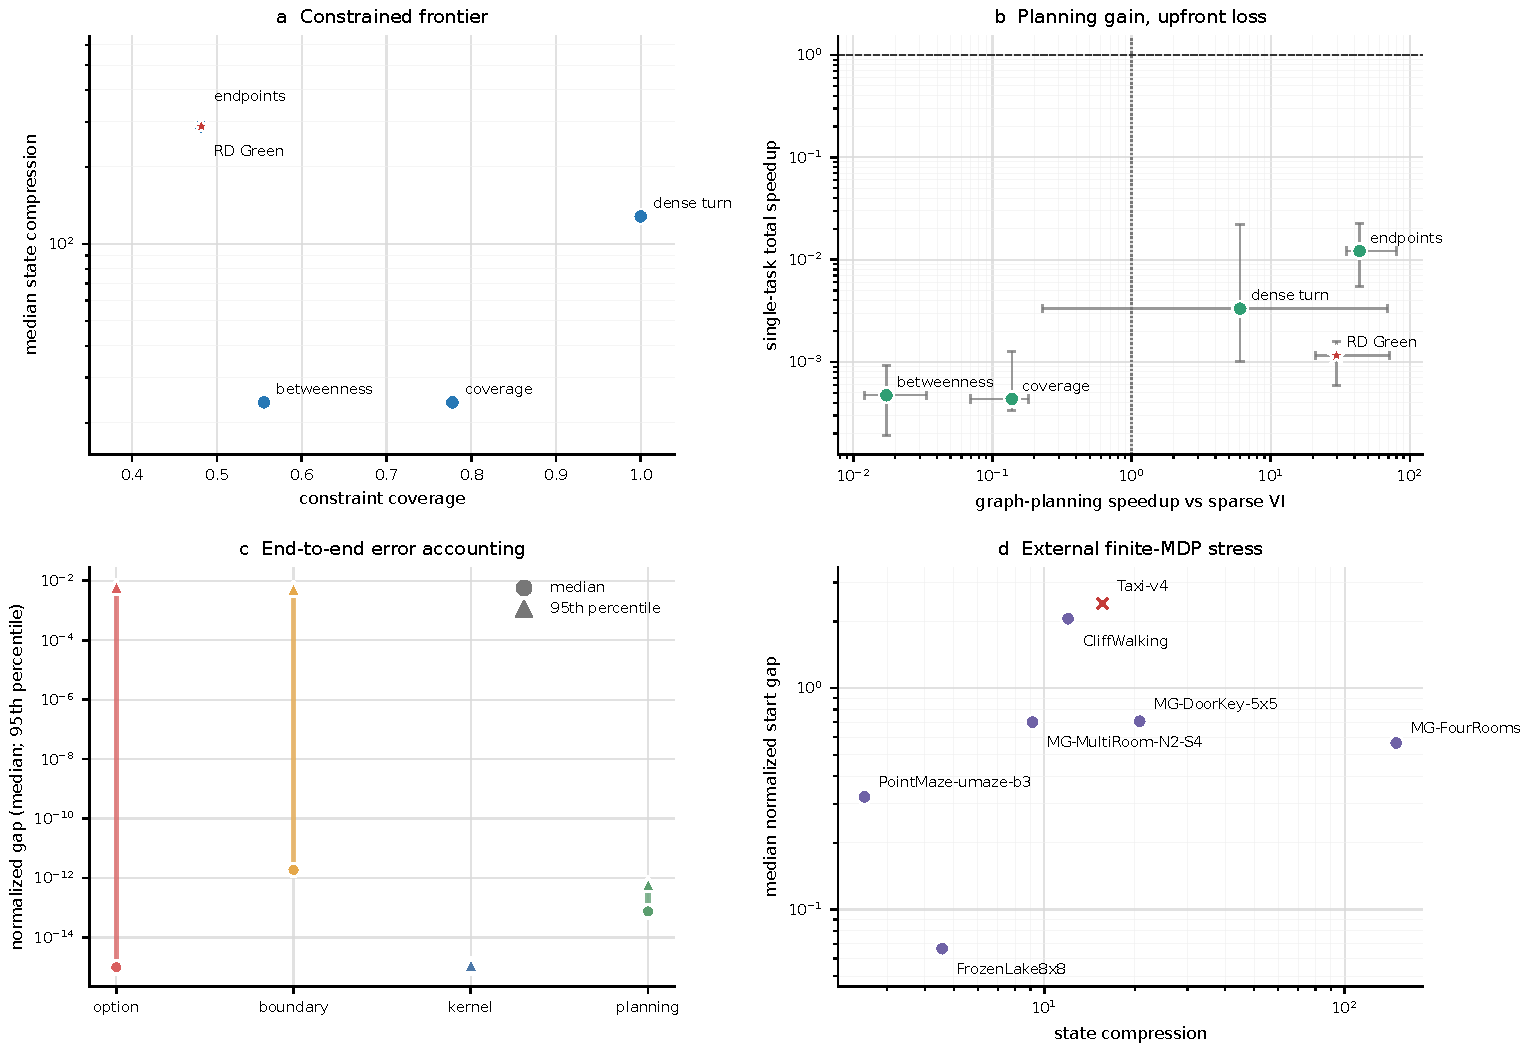
\includegraphics[width=\linewidth]{../experiments/output/p0_submission_figures/p0_evidence_panel.pdf}
\caption{Reviewer-facing evidence summary. (a) The canonical large-scale
frontier at normalized value gap $\leq0.01$ and normalized audit
$\leq0.001$; higher and farther right is better, but no selector dominates.
(b) Matched sparse-VI accounting separates graph-planning speedup from
single-task total time; bars are bootstrap 95\% intervals across cases.
(c) Median and 95th-percentile terms in the converged
primitive-to-graph decomposition; kernel and planning terms are numerical while
option/boundary tails remain. (d) Five-seed external finite-MDP stress tests;
Taxi-v4 is marked as a structured failure.}
\label{fig:p0-evidence}
\end{figure}

\begin{figure}[H]
\centering
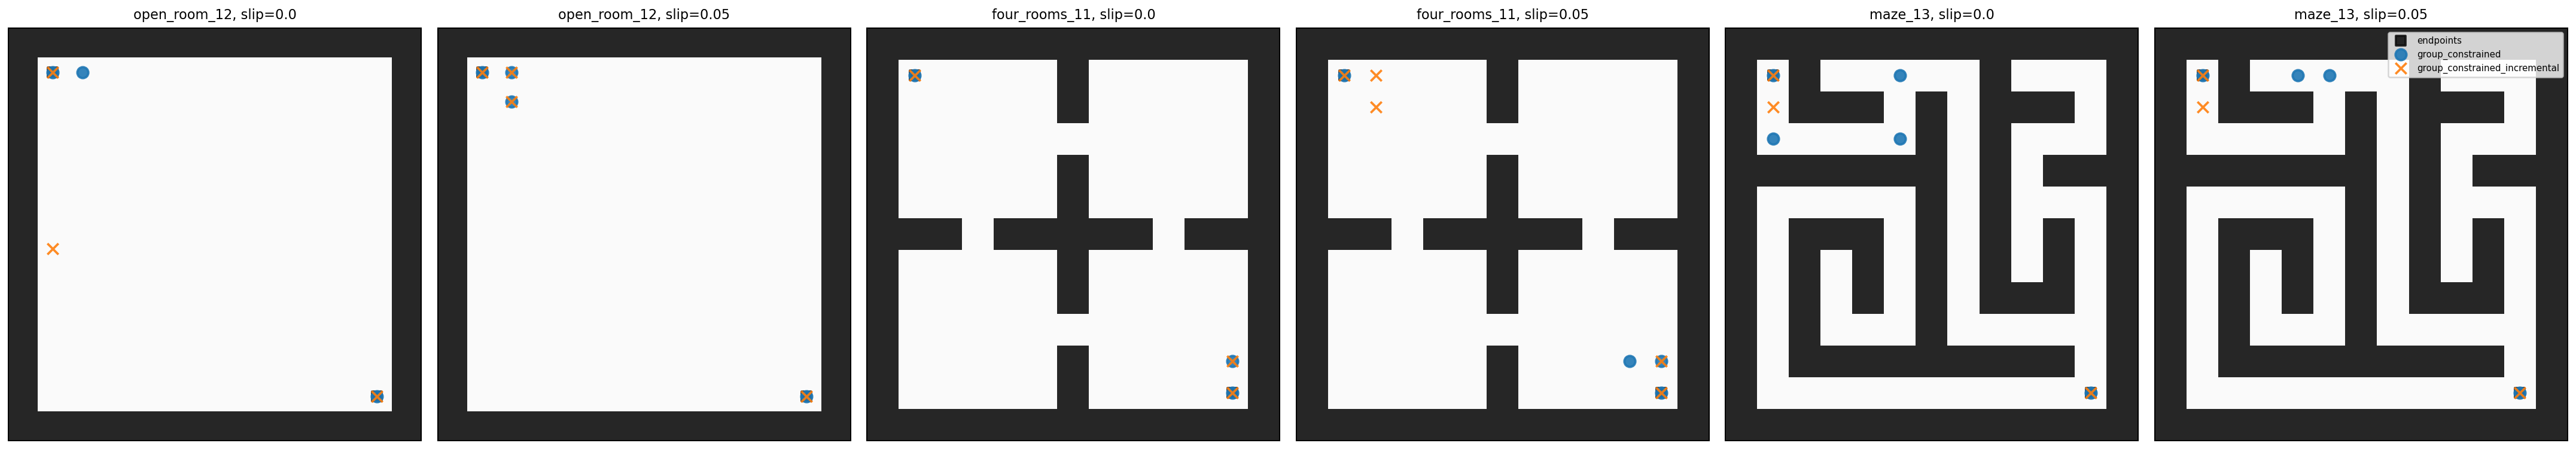
\includegraphics[width=\linewidth]{../experiments/output/graph_abstraction_figures/boundary_selection_panel.png}
\caption{Boundary overlays for open room, four rooms, and maze maps at slip
$0$ and $0.05$. Squares are mandatory endpoints; circles and crosses show
group-constrained and incremental selections. The figure is interpretability
evidence, not a runtime comparison: selected vertices expose doorways, turns,
or stochastic interfaces that endpoint-only edges can hide.}
\label{fig:boundaries}
\end{figure}

\section{Formal Verification}
The Lean 4 development separates finite/scaled statements from a Mathlib-backed
real-valued layer. It checks the frozen finite-difference identity, legality and
nonnegativity of finite first-hit kernels, finite Neumann-tail and weighted
certificates, bits-distortion curvature bounds, graph-SMDP contraction,
residual-to-value bounds, interval and top-set decisions, group feasibility,
adaptive feasible top-$k$, one-shot linear-channel error and threshold/local-
maximum stability, reward relabeling, goal-event error, and the four-term
primitive-to-graph gap. Formalization does not turn the adaptive discovery
or one-shot threshold heuristic into a global optimizer; it fixes the meaning
of the operators and their certificates.

\section{Limitations}
The current method assumes a finite known transition model or an explicitly
constructed empirical finite MDP. The proofs apply to that finite model, not
directly to an underlying continuous simulator. Boundary discovery can cost
more than one full-state solve when iterative search is used. The one-shot path
removes that search but can return a denser graph or fail a group audit; its
threshold is a model-selection parameter, not an RD-optimality theorem. Group constraints are only as complete as their
probe families. Taxi demonstrates that a spatial boundary graph may erase
factored task variables; resolving that case requires a compositional state
representation, not merely more spatial landmarks. Finally, adaptive feasible
top-$k$ preserves a fixed-prefix feasible envelope but is not an RD-optimal
split oracle without score-interval dominance. A future systems-oriented claim
would also require repeated graph-construction timings on fixed hardware; the
present paper uses deterministic backup/memory accounting and treats wall time
as a secondary audit.

\section{Conclusion}
The RD Boundary Green Operator turns boundary-graph construction into an
auditable rate-distortion problem. Exact first-boundary reductions explain how
interior regions become option edges; group constraints and certified adaptive
approximations expose where that compression fails. The resulting theory and
experiments support a bounded contribution: finite known-model planning can be
compressed onto a sparse boundary graph while separately accounting for option
restriction, abstraction, kernel, and planning errors. The one-shot transform
removes combinatorial boundary search, but exact final-edge construction remains
the single-task bottleneck. Extending this operator to sample-based or factored
settings remains outside the present claim.

\section*{Reproducibility Statement}
Code, locked dependencies, experiment entry points, scheduler shard manifests,
tracked CSV artifacts, and Lean sources are provided in the accompanying
repository. Heavy raw scheduler directories are excluded from version control;
their aggregated paper-facing tables are tracked. Every main theorem is mapped
to a Lean symbol and an experiment artifact in the theorem-to-experiment bridge.
The repository also checks citation keys, figure paths, labels, and central
numeric claims against tracked CSV artifacts before regenerating the manuscript.

\appendix

\section{One-Shot Operator Configuration}
\label{app:configuration}
Table~\ref{tab:one-shot-config} records the fixed operating point used for the
main one-shot rows. The distinction between the scoring prefix and final edge
model is intentional: the former is a single frozen transform, while the latter
uses the certified adaptive first-hit implementation after the boundary has
already been selected.

\begin{table}[H]
\centering
\caption{Paper-facing one-shot configuration. Channel values are clipped after
division by their positive-state 95th percentile within each graph.}
\label{tab:one-shot-config}
\footnotesize
\begin{tabular}{ll}
\toprule
Component & Configuration\\
\midrule
Mandatory boundary / anchors & task start and terminal endpoints\\
Candidate universe & turn or articulation states; one-hop endpoint exclusion\\
Response prefix & $K=256$, frontier tolerance $10^{-6}$, $\gamma=0.97$\\
Channels & exposure, Green curvature, control curvature, topology, entropy curvature\\
Selection & local maxima; support $q\geq2$; topology or stochastic gate\\
Operating point & $\tau=0.15$; at most 18 inserted vertices\\
Sensitivity & $\tau\in\{0.10,0.15,0.20\}$; random-maze stress at $0.75$\\
Final edge model & one certified adaptive first-hit kernel build\\
\bottomrule
\end{tabular}
\end{table}

\section{Learned Boundary-Proposal Ablations}
\label{app:learned}
The learned branch was a bounded falsification test of the stronger ``look once
and emit the graph'' hypothesis, not a second proposed method. The graph-only
reference suite contained 360 corridor, open-room, four-room, DFS-maze, and
braided-maze contexts at three slip levels, split into 180 training, 90
validation, and 90 strict scale-holdout contexts. A native sparse GCN
\citep{kipf2017gcn} used 28 observable transition, reward, topology, coordinate,
endpoint-distance, slip, and discount features. Five seeds were trained on
CUDA; validation selected one model and CPU inference because per-graph device
transfer outweighed GPU execution.

The single permitted follow-up froze five cheap proposal types: learned count,
top-1, top-2, top-3, and nearest-start. A train-only risk model predicted the
three group violations, normalized value gap, and joint failure, then reranked
the deduplicated family without candidate insertion, beam expansion, or Green
recomputation. The official validation split calibrated routing only; the scale
test was not used for model or epoch selection.

\begin{table}[H]
\centering
\caption{Learned proposal quality and acceptance cost on 90 strict scale
holdouts. ``Misses'' counts failed graphs that validation-calibrated routing did
not audit. Raw pass and candidate-oracle quality are not certificates.}
\label{tab:learned-ablation}
\footnotesize
\begin{tabular}{lrrrrrrl}
\toprule
Proposal & Raw pass & Oracle & Select speed & Audit cov. & Misses & Full audit & Certified\\
\midrule
Boundary-only GCN & 68/90 & -- & 769.8 & 40.0\% & 11/22 & 0.444 & no\\
Nearest-start & 62/90 & -- & 877.9 & -- & -- & 0.435 & no\\
Constraint-aware reranker & 81/90 & 85/90 & 656.0 & 14.4\% & 6/9 & 0.428 & no\\
Adaptive RD reference & 71/90 & -- & 1.0 & audit/cert. & -- & 1.0 & conditional\\
Candidate-family oracle & 85/90 & 85/90 & -- & -- & -- & -- & not deployable\\
\bottomrule
\end{tabular}
\end{table}

For the reranker/reference pairing, 64 contexts passed under both proposals, 17
under only the reranker, 7 under only the adaptive reference, and 2 under
neither. The pass-rate difference was 11.1 percentage points with a paired
bootstrap 95\% interval of 1.1 to 21.1 points; the exact conditional McNemar
test gave $p=0.0639$. The comparison remains descriptive because the objectives
and acceptance guarantees differ. Validation routing missed six of nine
reranker failures, and full audit was slower than the explicit reference
pipeline. The predefined go/no-go protocol therefore stopped the learned branch
before a further constraint-aware topology expansion.

\begingroup
\small
\setlength{\bibsep}{1pt}
\bibliographystyle{plainnat}
\bibliography{references}
\endgroup

\end{document}
